\section{La programmation orientée objet}
\begin{frame}
	\begin{center}
	\huge
	La programmation orientée objet
	\end{center}
\end{frame}

\subsection{Notion d'objet} %%%%%%%%%%%%%%%%%%%%%%%%%%%%%%%%%%%%%%%%%
\begin{frame}
	\frametitle{Comme une boite}
	\begin{center}
	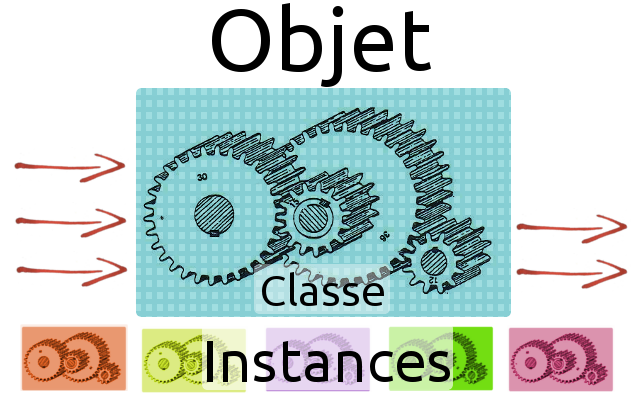
\includegraphics[width=9cm]{pics/explObj1.png}
	\end{center}
\end{frame}
\begin{frame}
	\frametitle{Attributs/Méthodes}
	\begin{center}
	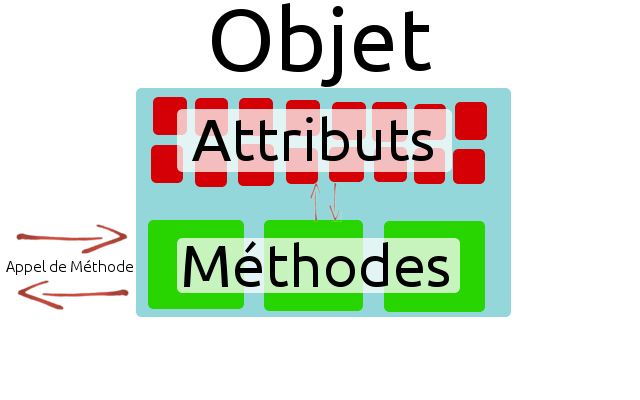
\includegraphics[width=9cm]{pics/explObj2.png}
	\end{center}
\end{frame}
\begin{frame}[fragile]
	\frametitle{Exemple d'utilisation d'objet}
	\begin{lstlisting}
let (c1,c2) =
  let m1 = new CoffeMachine(Bresile)
  and m2 = new CoffeMachine(Islande)
  in let _ = 
    m1#addWater(1000);
    m2#addWater(42000)
  in let _ =
    m1#headUp();
    m2#headUp()
  in (m1#getCoffe(1),m2#getCoffe(3))
;;
	\end{lstlisting}
\end{frame}

\subsection{La déclaration d'un objet} %%%%%%%%%%%%%%%%%%%%%%%%%%%%%%
\begin{frame}[fragile]
	\frametitle{Syntaxe}
	\begin{minipage}{0.45\textwidth}
		\lstset{basicstyle=\small}
		\begin{lstlisting}
class name parameters =
  object
    (*Attributs*)
    
    (*Methods*)
  end
		\end{lstlisting}
	\end{minipage}
	\begin{minipage}{0.4\textwidth}
		\begin{lstlisting}
class point x y =
  object
    val x = x
    val y = y

    method printCoord =
      print_int x;
      print_string ",";
      print_int y;
      print_string "\n"
  end
		\end{lstlisting}
	\end{minipage}
\end{frame}

\begin{frame}[fragile]
	\frametitle{Déclaration d'attribut}
	\textit{Tenez vous à un type}\\
	\textbf{Simple}
	\begin{lstlisting}
  val name = expr
	\end{lstlisting}
	\textbf{Modifiable}
	\begin{lstlisting}
  val mutable name = expr
  name <- expr
	\end{lstlisting}
	\textbf{Lorsque rien ne marche : Le type Option}
	\begin{lstlisting}
  val mutable name = None
  name <- Some expr
	\end{lstlisting}
\end{frame}

\begin{frame}[fragile]
	\frametitle{Déclaration de méthode}
	\textbf{simple}
	\begin{lstlisting}
  method name parameters = expr
	\end{lstlisting}
	\textbf{privée}\\
	\begin{minipage}{0.4\textwidth}
  	\begin{lstlisting}
  class name =
    object
    ...
    end
		\end{lstlisting}
	\end{minipage}$\Rightarrow$
	\begin{minipage}{0.4\textwidth}
		\begin{lstlisting}
  class name =
    object (self)
    ...
    end
		\end{lstlisting}
	\end{minipage}
	\begin{lstlisting}
  method private name parameters = expr
  self#privateMethod parameters
	\end{lstlisting}
\end{frame}

\begin{frame}[fragile]
	\frametitle{Initialisation}
	\begin{lstlisting}
class putLineInQueue (l:int list) =
  object (self)
    
  val data = Queue.create ()

  initializer
    let rec storage = function
      | [] -> ()
      | e::q -> 
        push e data;
        storage q
    in storage l

  ...
  end
	\end{lstlisting}
\end{frame}

\begin{frame}[fragile]
	\frametitle{Attributs polymorphiques}
	\begin{lstlisting}
class ['a] name parameters =
  object 
  val data = ref []

  method add e =
    data := e::!data
  
  ...
  end
	\end{lstlisting}
\end{frame}

\subsection{L'heritage} %%%%%%%%%%%%%%%%%%%%%%%%%%%%%%%%%%%%%%%%%%%%%
\begin{frame}[fragile]
	\frametitle{Syntaxe de l'heritage}
	\begin{lstlisting}
class childName parameters =
  object
  inherit motherClass mothersParameters

  end
	\end{lstlisting}
	\begin{lstlisting}
class childName parameters =
  object
  inherit motherClass mothersParameters 
    as motherSelf

  end
	\end{lstlisting}
\end{frame}

\begin{frame}
	\frametitle{Accès aux méthodes de la classe mère 1/2}
	\lstinputlisting[firstline=1, lastline=14]{code/heritage.ml}
\end{frame}

\begin{frame}
	\frametitle{Accès aux méthodes de la classe mère 2/2}
	\textit{Le type d'une réécritrue d'une méthode doit correspondre à celui de la méthode mère.}
	\lstinputlisting[firstline=16, lastline=28]{code/heritage.ml}
\end{frame}
\subsection{Le polymorphisme d'inclusion} %%%%%%%%%%%%%%%%%%%%%%%%%%%
\begin{frame}
	\frametitle{Le polymorphisme de sous-inclusion}
	\begin{center}
		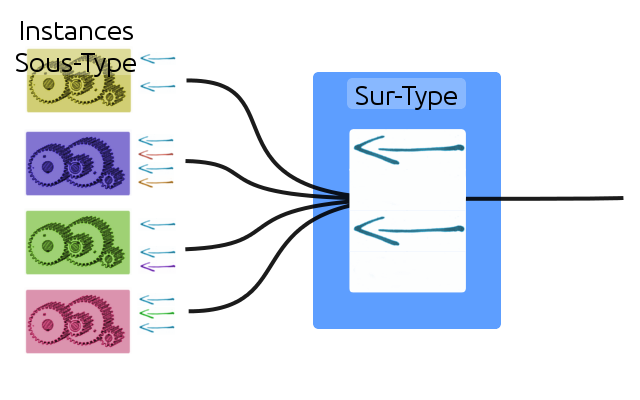
\includegraphics[width=9cm]{pics/inclusionObjet.png}
	\end{center}
\end{frame}

\begin{frame}[fragile]
	\frametitle{Interface et opérateur de sous-type}
	\textit{Le type des méthodes doit correspondres à celui de la méthode de l'interface.}\\
	\begin{center}
		\begin{minipage}{0.4\textwidth}
			\lstset{basicstyle=\scriptsize}
  		\begin{lstlisting}
  class c1 =
    object
    method m1 = ...
    method ma = ...
    method m2 = ...
    method mb = ...
    end
			\end{lstlisting}
		\end{minipage}
		\begin{minipage}{0.4\textwidth}
		  \lstset{basicstyle=\scriptsize}
			\begin{lstlisting}
  class c2 =
    object (self)
    method mc = ...
    method m2 = ...
    method md = ...
    method m1 = ...
    end
			\end{lstlisting}
		\end{minipage}
	\end{center}
	\begin{center}
		\begin{minipage}{0.4\textwidth}
			\lstset{basicstyle=\footnotesize}
			\begin{lstlisting}
class type i1 =
  object
    method m1 : string
    method m2 : int list
  end
			\end{lstlisting}
		\end{minipage}
		\begin{minipage}{0.4\textwidth}
			\lstset{basicstyle=\scriptsize}
			\begin{lstlisting}
    let a = (new c1):>i1
    and b = (new c2):>i1
			\end{lstlisting}
		\end{minipage}
	\end{center}
\end{frame}

\begin{frame}[fragile]
	\frametitle{Exemple d'utilisation du sous-polymorphisme d'inclusion}
	Réutilisons les class point et colored\_point.
	\begin{lstlisting}
  let f (o:point) = o#setCoord 4 2
  let test = 
    ((new colored_point (4,2) 255):>point)

  test#print
  f test
  test#print
  test#setData 4 5 1
	\end{lstlisting}
	\textbf{Sortie :}
	\begin{lstlisting}
  (2,4) 255
  (4,2) 255
  Error: This expression has type point
         It has no method setData
	\end{lstlisting}
\end{frame}
